
\section{\label{sec:UndeterminedCoefficients}Koefisien Tak Tentu\index{koefisien tak tentu}}

\subsection{Gagasan dasar}

Menurut persamaan \ref{eq:lagrangeInterpolatingPolynomialError},
selisih antara $f$ dan suatu polinom interpolasi merupakan kelipatan
dari $f^{(n+1)}(\xi_{x})$. Dengan kata lain, galat dalam mengaproksimasi
$f$ dengan polinom interpolasi $P_{n}$ bergantung langsung pada
$f^{(n+1)}$. Namun, $f^{(n+1)}(x)$ identik nol setiap kali $f$
merupakan polinom berderajat kurang dari $n+1$. Akibatnya, $(f-P_{n})(x)$
identik nol dalam kasus ini. Meskipun terdengar berulang, gagasan
terakhir ini layak ditegaskan kembali. Jika $f$ adalah sembarang
polinom berderajat kurang dari $n+1$, maka $P_{n}$, yang dihitung
untuk sembarang himpunan yang terdiri dari $n+1$ simpul, sama persis
dengan $f$ untuk semua $x$. Dengan demikian, turunan $P_{n}$ dan
integral $P_{n}$ bukan sekadar aproksimasi terhadap turunan dan integral
yang bersesuaian dari $f$. Keduanya eksak karena $P_{n}=f$ untuk
semua $x$. Pengamatan ini dapat digunakan untuk menurunkan rumus
turunan dan integral tanpa pernah menghitung $P_{n}$ maupun turunan
atau integralnya!

Semua rumus yang telah kita turunkan untuk mengaproksimasi turunan
dan integral dari fungsi sembarang $f$ berbentuk
\[
\sum_{i=0}^{n}a_{i}f(x_{i})
\]
dengan $x_{0},x_{1},\ldots,x_{n}$ adalah simpul-simpul polinom interpolasi,
yaitu titik-titik tempat nilai $f$ diketahui, sedangkan $a_{i}$
adalah konstanta yang diperoleh dari penurunan tersebut. Metode koefisien
tak tentu menggunakan pendekatan langsung untuk menghitung konstanta
$a_{i}$. Dengan mengetahui bahwa rumus ``aproksimasi'' harus eksak
untuk semua polinom berderajat $0,1,\ldots,n$, kita dapat membentuk
$n+1$ persamaan dengan $n+1$ peubah tak diketahui, yaitu $a_{0},a_{1},\ldots,a_{n}$.
Penyelesaian sistem persamaan yang dihasilkan memberikan nilai koefisien
tersebut.

\subsection{Turunan\index{diferensiasi numerik}}

Kita mencari aproksimasi untuk turunan orde $k$ dari $f$ berdasarkan
nilai-nilai yang diketahui, yaitu $f(x_{0}+\theta_{0}h),f(x_{0}+\theta_{1}h),\ldots,f(x_{0}+\theta_{n}h)$.
Secara tepat, kita menginginkan aproksimasi berbentuk
\begin{equation}
f^{(k)}(x_{0}+\theta h)\approx\sum_{i=0}^{n}a_{i}f(x_{0}+\theta_{i}h).\label{eq:derivApprox}
\end{equation}
Berdasarkan persamaan \ref{eq:lagrangeInterpolatingPolynomialError},
aproksimasi tersebut harus eksak untuk semua polinom berderajat $n$
atau kurang. Secara khusus, aproksimasi itu harus eksak untuk polinom
$p_{j}(x)=(x-x_{0})^{j}$, $j=0,1,\ldots,n$. Secara simbolis, harus
berlaku
\[
p_{j}^{(k)}(x_{0}+\theta h)=\sum_{i=0}^{n}a_{i}p_{j}(x_{0}+\theta_{i}h)
\]
untuk $j=0,1,\ldots,n$. Perhatikan bahwa aproksimasi tersebut kini
menjadi suatu kesamaan \textit{eksak}. Dengan memperhatikan bahwa
$p_{j}(x_{0}+\theta_{i}h)=((x_{0}+\theta_{i}h)-x_{0})^{j}=(\theta_{i}h)^{j}$,
sistem persamaan tersebut menjadi
\begin{equation}
p_{j}^{(k)}(x_{0}+\theta h)=a_{0}+\sum_{i=1}^{n}(\theta_{i}h)^{j}a_{i}\label{eq:systemGenericDerivative}
\end{equation}
untuk $j=0,1,\ldots,n$. Penyelesaian sistem inilah yang akan menghasilkan
$a_{i}$.

\noindent\begin{digression}{Matriks Vandermonde}

\noindent Secara umum, suatu sistem persamaan linear mungkin memiliki
nol, satu, atau banyak penyelesaian. Namun, sistem \ref{eq:systemGenericDerivative}
memiliki bentuk khusus. Dalam setiap persamaan, konstanta $(\theta_{i}h)^{j}$
membentuk barisan geometri. Matriks koefisien seperti ini disebut
matriks Vandermonde, dan diketahui bahwa selama $\theta_{i}$ saling
berbeda, sistem ini akan memiliki satu penyelesaian. 

\noindent\end{digression}

Sebagai ilustrasi, misalkan kita memiliki stensil 

\begin{center}
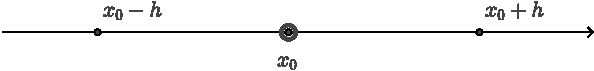
\includegraphics{figures/calculus-rudiments03}
\par\end{center}

\noindent dan kita ingin memperoleh rumus untuk turunan pertama dan
kedua dari $f$ (pada $x_{0}$). Untuk stensil ini, $\theta=0$, $\theta_{0}=-1$,
$\theta_{1}=0$, serta $\theta_{2}=1$, sehingga kita mencari rumus
dengan bentuk
\begin{eqnarray*}
f'(x_{0}) & \approx & a_{0}f(x_{0}-h)+a_{1}f(x_{0})+a_{2}f(x_{0}+h)\\
 &  & \mbox{ dan}\\
f''(x_{0}) & \approx & b_{0}f(x_{0}-h)+b_{1}f(x_{0})+b_{2}f(x_{0}+h).
\end{eqnarray*}
Masing-masing rumus ini harus eksak ketika $f=p_{0}$, ketika $f=p_{1}$,
dan ketika $f=p_{2}$. Ketiga syarat ini menghasilkan tiga persamaan
dengan tiga peubah tak diketahui.

Dimulai dari rumus turunan pertama, kita merinci sistem \ref{eq:systemGenericDerivative}
dengan $k=1$ dan $n=2$:
\begin{eqnarray*}
p_{0}'(x_{0}) & = & a_{0}p_{0}(x_{0}-h)+a_{1}p_{0}(x_{0})+a_{2}p_{0}(x_{0}+h)\\
p_{1}'(x_{0}) & = & a_{0}p_{1}(x_{0}-h)+a_{1}p_{1}(x_{0})+a_{2}p_{1}(x_{0}+h)\\
p_{2}'(x_{0}) & = & a_{0}p_{2}(x_{0}-h)+a_{1}p_{2}(x_{0})+a_{2}p_{2}(x_{0}+h)
\end{eqnarray*}
Menurut definisi, $p_{0}(x)=(x-x_{0})^{0}=1$ sehingga $p_{0}'(x_{0})=0$;
$p_{1}(x)=(x-x_{0})^{1}=x-x_{0}$ sehingga $p_{1}'(x_{0})=1$; dan
$p_{2}(x)=(x-x_{0})^{2}$ sehingga $p_{2}'(x)=2(x-x_{0})$ yang menghasilkan
$p_{2}'(x_{0})=0$. Dengan menyubstitusikan informasi ini ke dalam
persamaan di atas,
\begin{eqnarray*}
0 & = & a_{0}+a_{1}+a_{2}\\
1 & = & -ha_{0}+ha_{2}\\
0 & = & h^{2}a_{0}+h^{2}a_{2}.
\end{eqnarray*}
Sistem ini dapat diselesaikan dengan substitusi, eliminasi, atau bantuan
sistem aljabar komputer. Penyelesaiannya adalah $a_{0}=\frac{-1}{2h}$,
$a_{1}=0$, dan $a_{2}=\frac{1}{2h}$, sehingga diperoleh rumus aproksimasi
\[
f'(x_{0})\approx\frac{f(x_{0}+h)-f(x_{0}-h)}{2h}
\]
seperti yang telah kita peroleh \vpageref{eq:centeredDifferenceNaive}
dalam rumus \ref{eq:centeredDifferenceNaive}.

Rumus turunan kedua diturunkan dengan cara yang sama. Karena rumus
turunan kedua harus eksak ketika $f=p_{0}$, ketika $f=p_{1}$, dan
ketika $f=p_{2}$, nilai-nilai $a_{i}$ harus memenuhi
\begin{eqnarray*}
p_{0}''(x_{0}) & = & b_{0}p_{0}(x_{0}-h)+b_{1}p_{0}(x_{0})+b_{2}p_{0}(x_{0}+h)\\
p_{1}''(x_{0}) & = & b_{0}p_{1}(x_{0}-h)+b_{1}p_{1}(x_{0})+b_{2}p_{1}(x_{0}+h)\\
p_{2}''(x_{0}) & = & b_{0}p_{2}(x_{0}-h)+b_{1}p_{2}(x_{0})+b_{2}p_{2}(x_{0}+h),
\end{eqnarray*}
sistem \ref{eq:systemGenericDerivative} dengan $k=2$ dan $n=2$.
Perhatikan bahwa ruas kanan persis sama dengan ruas kanan pada rumus
turunan pertama, kecuali perubahan nama dari $a_{i}$ menjadi $b_{i}$.
Hanya ruas kiri yang berubah secara substantif. $p_{0}''(x)=0$ sehingga
$p_{0}''(x_{0})=0$; $p_{1}''(x)=0$ sehingga $p_{1}(x_{0})=0$; dan
$p_{2}''(x)=2$ sehingga $p_{2}''(x_{0})=2$. Dengan melakukan substitusi
ini ke dalam persamaan di atas,
\begin{eqnarray*}
0 & = & b_{0}+b_{1}+b_{2}\\
0 & = & -hb_{0}+hb_{2}\\
2 & = & h^{2}b_{0}+h^{2}b_{2}.
\end{eqnarray*}
Sekali lagi, sistem ini dapat diselesaikan dengan substitusi, eliminasi,
atau bantuan sistem aljabar komputer. Penyelesaiannya adalah $b_{0}=b_{2}=\frac{1}{h^{2}}$
dan $b_{1}=\frac{2}{h^{2}}$, sehingga diperoleh rumus aproksimasi
\[
f''(x_{0})\approx\frac{f(x_{0}+h)-2f(x_{0})+f(x_{0}-h)}{h^{2}}.
\]


\subsection{Integral\index{integrasi numerik}}

Gagasan untuk memperkirakan integral sama persis dengan gagasan untuk
memperkirakan turunan. Hanya mekanismenya yang berubah sedikit. Jika
sebelumnya terdapat turunan, kini kita akan menggunakan integral.
Kita mencari aproksimasi untuk $\int_{a}^{b}f(x)dx$ berdasarkan nilai-nilai
yang diketahui, yaitu $f(x_{0}+\theta_{0}h),f(x_{0}+\theta_{1}h),\ldots,f(x_{0}+\theta_{n}h)$:
\begin{equation}
\int_{a}^{b}f(x)dx\approx\sum_{i=0}^{n}a_{i}f(x_{0}+\theta_{i}h).\label{eq:integralApprox}
\end{equation}
Aproksimasi tersebut akan eksak untuk semua polinom berderajat $n$
atau kurang. Secara khusus, aproksimasi itu akan eksak untuk $p_{j}(x)=(x-x_{0})^{j}$,
$j=0,1,\ldots,n$. Oleh karena itu, sistem persamaan
\begin{equation}
\int_{a}^{b}p_{j}(x)dx=a_{0}+\sum_{i=1}^{n}(\theta_{i}h)^{j}a_{i}\qquad j=0,1,\ldots,n\label{eq:systemGenericIntegral}
\end{equation}
harus dipenuhi oleh $a_{i}$.

Sebagai ilustrasi, misalkan kita memiliki stensil 

\begin{center}
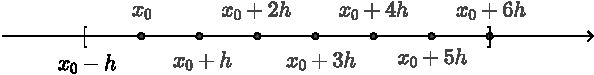
\includegraphics{figures/calculus-rudiments05}.
\par\end{center}

\noindent Untuk stensil ini, $a=x_{0}-h$, $b=x_{0}+6h$, dan $\theta_{i}=ih$,
$i=0,1,\ldots,6$. Dengan demikian, kita akan memperoleh sistem tujuh
persamaan dengan tujuh peubah tak diketahui. Pertama, ruas kirinya:

\begin{eqnarray*}
\int_{a}^{b}p_{0}(x)dx=\int_{x_{0}-h}^{x_{0}+6h}p_{0}(x)dx & = & \int_{x_{0}-h}^{x_{0}+6h}1dx=\left.(x-x_{0})\right|_{x_{0}-h}^{x_{0}+6h}=7h\\
\int_{a}^{b}p_{1}(x)dx=\int_{x_{0}-h}^{x_{0}+6h}p_{1}(x)dx & = & \int_{x_{0}-h}^{x_{0}+6h}(x-x_{0})dx=\left.\frac{1}{2}(x-x_{0})^{2}\right|_{x_{0}-h}^{x_{0}+6h}=\frac{35}{2}h^{2}\\
\int_{a}^{b}p_{2}(x)dx=\int_{x_{0}-h}^{x_{0}+6h}p_{2}(x)dx & = & \int_{x_{0}-h}^{x_{0}+6h}(x-x_{0})^{2}dx=\left.\frac{1}{3}(x-x_{0})^{3}\right|_{x_{0}-h}^{x_{0}+6h}=\frac{217}{3}h^{3}\\
\int_{a}^{b}p_{3}(x)dx=\int_{x_{0}-h}^{x_{0}+6h}p_{3}(x)dx & = & \int_{x_{0}-h}^{x_{0}+6h}(x-x_{0})^{3}dx=\left.\frac{1}{4}(x-x_{0})^{4}\right|_{x_{0}-h}^{x_{0}+6h}=\frac{1295}{4}h^{4}\\
\int_{a}^{b}p_{4}(x)dx=\int_{x_{0}-h}^{x_{0}+6h}p_{4}(x)dx & = & \int_{x_{0}-h}^{x_{0}+6h}(x-x_{0})^{4}dx=\left.\frac{1}{5}(x-x_{0})^{5}\right|_{x_{0}-h}^{x_{0}+6h}=\frac{7777}{5}h^{5}\\
\int_{a}^{b}p_{5}(x)dx=\int_{x_{0}-h}^{x_{0}+6h}p_{5}(x)dx & = & \int_{x_{0}-h}^{x_{0}+6h}(x-x_{0})^{5}dx=\left.\frac{1}{6}(x-x_{0})^{6}\right|_{x_{0}-h}^{x_{0}+6h}=\frac{46655}{6}h^{6}\\
\int_{a}^{b}p_{6}(x)dx=\int_{x_{0}-h}^{x_{0}+6h}p_{6}(x)dx & = & \int_{x_{0}-h}^{x_{0}+6h}(x-x_{0})^{6}dx=\left.\frac{1}{7}(x-x_{0})^{7}\right|_{x_{0}-h}^{x_{0}+6h}=39991h^{7}.
\end{eqnarray*}
Sekarang kita gabungkan semuanya dengan ruas kanan (dan menukar ruas):
\begin{eqnarray*}
\sum_{i=0}^{6}(\theta_{i}h)^{0}a_{i} & = & a_{0}+a_{1}+a_{2}+a_{3}+a_{4}+a_{5}+a_{6}=7h\\
\sum_{i=0}^{6}(\theta_{i}h)^{1}a_{i} & = & ha_{1}+2ha_{2}+3ha_{3}+4ha_{4}+5ha_{5}+6ha_{6}=\frac{35}{2}h^{2}\\
\sum_{i=0}^{6}(\theta_{i}h)^{2}a_{i} & = & h^{2}a_{1}+4h^{2}a_{2}+9h^{2}a_{3}+16h^{2}a_{4}+25h^{2}a_{5}+36h^{2}a_{6}=\frac{217}{3}h^{3}\\
\sum_{i=0}^{6}(\theta_{i}h)^{3}a_{i} & = & h^{3}a_{1}+8h^{3}a_{2}+27h^{3}a_{3}+64h^{3}a_{4}+125h^{3}a_{5}+216h^{3}a_{6}=\frac{1295}{4}h^{4}\\
\sum_{i=0}^{6}(\theta_{i}h)^{4}a_{i} & = & h^{4}a_{1}+16h^{4}a_{2}+81h^{4}a_{3}+256h^{4}a_{4}+625h^{4}a_{5}+1296h^{4}a_{6}=\frac{7777}{5}h^{5}\\
\sum_{i=0}^{6}(\theta_{i}h)^{5}a_{i} & = & h^{5}a_{1}+32h^{5}a_{2}+243h^{5}a_{3}+1024h^{5}a_{4}+3125h^{5}a_{5}+7776h^{5}a_{6}=\frac{46655}{6}h^{6}\\
\sum_{i=0}^{6}(\theta_{i}h)^{6}a_{i} & = & h^{6}a_{1}+64h^{6}a_{2}+729h^{6}a_{3}+4096h^{6}a_{4}+15625h^{6}a_{5}+46656h^{6}a_{6}=39991h^{7}
\end{eqnarray*}
Sekali lagi, sistem ini dapat diselesaikan dengan substitusi, eliminasi,
atau aljabar komputer, setidaknya secara prinsip. Namun, tidak banyak
orang yang memiliki cukup kesabaran dan ketelitian untuk menyelesaikan
sistem seperti itu dengan kertas dan pensil. Dengan mengandalkan sistem
aljabar komputer, penyelesaiannya adalah $a_{0}=\frac{30919}{8640}h$,
$a_{1}=-\frac{2107}{360}h$, $a_{2}=\frac{34153}{2880}h$, $a_{3}=-\frac{1274}{135}h$,
$a_{4}=\frac{19943}{2880}h$, $a_{5}=-\frac{49}{72}h$, dan $a_{6}=\frac{5257}{8640}h$
sehingga diperoleh rumus aproksimasi
\begin{eqnarray}
\int_{x_{0}-h}^{x_{0}+6h}f(x)dx & \approx & \frac{h}{8640}\left[5257f(x_{0}+6h)-5880f(x_{0}+5h)+59829f(x_{0}+4h)-81536f(x_{0}+3h)\right.\nonumber \\
 &  & \qquad\qquad\left.+102459f(x_{0}+2h)-50568f(x_{0}+h)+30919f(x_{0})\right]\label{eq:dumbIntegral7}
\end{eqnarray}
seperti yang telah kita peroleh \vpageref{eq:integral7dumb} dalam
rumus \ref{eq:integral7dumb}.

\subsection{Pertimbangan praktis}

Kita telah menggunakan stensil seperti 

\begin{center}
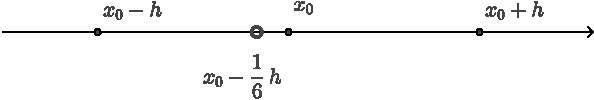
\includegraphics{figures/calculus-rudiments01}
\par\end{center}

\noindent dan 

\begin{center}
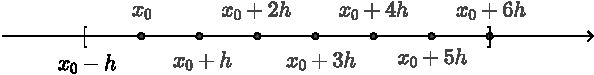
\includegraphics{figures/calculus-rudiments05}
\par\end{center}

\noindent bukan karena hasilnya sangat berguna, melainkan untuk (a)
mengilustrasikan metode tersebut dan (b) menekankan bahwa metode ini
berlaku secara umum untuk setiap stensil yang dapat Anda bayangkan.
Sebagian besar rumus diferensiasi dan integrasi dalam literatur analisis
numerik hanya menggunakan sejumlah kecil stensil berjarak teratur.
Untuk turunan, titik evaluasinya merupakan salah satu simpul; untuk
integral, semua simpul berada di antara kedua batas atau terdapat
simpul pada kedua batas. Mungkin saja hanya stensil berjarak teratur
yang akan Anda perlukan, tetapi ada baiknya mengetahui bahwa Anda
dapat menurunkan rumus yang sesuai untuk stensil yang tidak lazim
jika diperlukan.

Dalam hal penurunannya, keunggulan utama metode koefisien tak tentu
dibandingkan bekerja langsung dengan polinom interpolasi adalah kemudahan
otomasi serta berkurangnya pekerjaan aljabar yang sering kali rumit
dan melelahkan. Dalam metode koefisien tak tentu, satu-satunya polinom
yang perlu diturunkan atau diintegralkan adalah polinom $p_{j}=(x-x_{0})^{j}$,
tugas yang jauh lebih sederhana daripada mengintegralkan atau menurunkan
polinom interpolasi. Rumus dengan tiga atau empat simpul dapat ditangani
dengan cara ini menggunakan pensil dan kertas. Konsekuensinya adalah
perlunya menyelesaikan suatu sistem persamaan, yang sekali lagi lebih
sederhana daripada menurunkan dan menyederhanakan polinom interpolasi
berderajat 3 atau 4. Keunggulan terakhir metode koefisien tak tentu
adalah bahwa metode ini merupakan teknik penyelesaian umum yang tidak
hanya digunakan dalam analisis numerik untuk menurunkan aproksimasi
kalkulus, tetapi juga dalam bidang lain, terutama dalam persamaan
diferensial. Metode ini dapat diterapkan kapan pun \textit{bentuk}
suatu penyelesaian atau rumus diketahui, tetapi konstantanya (koefisien)
masih belum diketahui.

\noindent\begin{digression}{Koefisien Tak Tentu dalam Persamaan Diferensial}

\noindent Dalam persamaan diferensial, kita mengetahui bahwa suatu
solusi khusus dari persamaan
\begin{equation}
y-2y'+3y''=5\sin x\label{eq:differentialEquation}
\end{equation}
berbentuk $y=A\sin x+B\cos x$, tetapi kita belum langsung mengetahui
nilai $A$ dan $B$. Keduanya merupakan koefisien tak tentu (pada
tahap ini). Koefisien tersebut ditentukan dengan menyubstitusikan
bentuk yang diketahui ke dalam persamaan yang sedang diselesaikan.
\begin{eqnarray*}
y' & = & A\cos x-B\sin x\\
y'' & = & -A\sin x-B\cos x
\end{eqnarray*}
Dengan demikian, persamaan yang sedang diselesaikan menjadi
\[
(A\sin x+B\cos x)-2(A\cos x-B\sin x)+3(-A\sin x-B\cos x)=5\sin x.
\]
Dengan mengumpulkan koefisien $\sin x$ dan $\cos x$ pada ruas kiri,
\[
(-2A+2B)\sin x+(-2A-2B)\cos x=5\sin x.
\]
Sekarang kita menyamakan koefisien pada ruas kiri dan kanan untuk
memperoleh sistem persamaan
\begin{eqnarray*}
-2A+2B & = & 5\\
-2A-2B & = & 0
\end{eqnarray*}
yang penyelesaiannya adalah $A=-\frac{5}{4}$ dan $B=\frac{5}{4}$.
Oleh karena itu, $y=-\frac{5}{4}\sin x+\frac{5}{4}\cos x$ merupakan
solusi persamaan \ref{eq:differentialEquation}.

Secara konseptual, proses ini tidak berbeda dari metode koefisien
tak tentu yang digunakan untuk menurunkan rumus kalkulus numerik.
Bentuk penyelesaian suatu masalah telah diketahui, kecuali beberapa
koefisien (yang belum ditentukan). Parameter masalah mengharuskan
koefisien tersebut memenuhi suatu sistem persamaan linear. Sistem
tersebut diselesaikan, sehingga solusi masalah semula akhirnya diketahui
secara lengkap karena koefisiennya telah ditentukan.

\noindent\end{digression}

Ketika kita menggunakan stensil dengan lebih dari 3 atau 4 simpul,
menyelesaikan sistem persamaan linear (yang relatif besar) yang dihasilkan
secara manual bukanlah tugas yang dinantikan oleh kebanyakan dari
kita. Namun, ini merupakan perhitungan standar yang dapat dilakukan
oleh setiap sistem aljabar komputer dengan mudah dan efisien. Memang,
sebaiknya kita menggunakan sistem aljabar komputer untuk menurunkan
rumus serumit \ref{eq:integral7dumb}. Kita telah menggunakan Maxima\footnote{Lihat \url{http://maxima.sourceforge.net/}}\index{Maxima}
untuk menangani atau memeriksa ulang sejumlah perhitungan yang lebih
melelahkan yang disajikan dalam buku ini.

\noindent\begin{digression}{wxMaxima}\index{wxMaxima}\index{Maxima}

\noindent Cara terbaik untuk menyelesaikan sistem persamaan linear
yang besar adalah dengan bantuan sistem aljabar komputer. Gambar \ref{fig:wxMaxima}
menunjukkan cara menggunakan wxMaxima untuk menurunkan rumus \ref{eq:dumbIntegral7}.

Perhatikan kemiripan antara kode Maxima dan kode Octave. Maxima mendukung
pernyataan, pernyataan cetak, penugasan variabel, larik, dan penyembunyian
keluaran. Sintaks untuk hal-hal tersebut tidak sama, tetapi prinsip
yang mendasarinya sama. Setelah Anda mempelajari cara melakukan hal-hal
tersebut dalam satu bahasa, mempelajari caranya dalam bahasa lain
biasanya mudah.

Perhatikan pula perbedaan utama antara Maxima dan Octave. Maxima dirancang
untuk manipulasi simbolik, sedangkan Octave dirancang untuk komputasi
numerik. Octave dapat digunakan untuk melakukan perhitungan simbolik
dan Maxima dapat digunakan untuk melakukan komputasi numerik, tetapi
pepatah lama tukang kayu ``gunakan alat yang tepat untuk pekerjaan
yang dihadapi'' patut dipertimbangkan. Maxima jauh lebih mahir dalam
manipulasi simbolik daripada Octave, sedangkan Octave jauh lebih mahir
dalam mengolah angka daripada Maxima.

\subsection*{Referensi}

\url{http://andrejv.github.io/wxmaxima/}

\noindent\end{digression} 
\begin{figure}
\caption{\label{fig:wxMaxima}Menurunkan rumus integrasi dengan wxMaxima}

\centering{}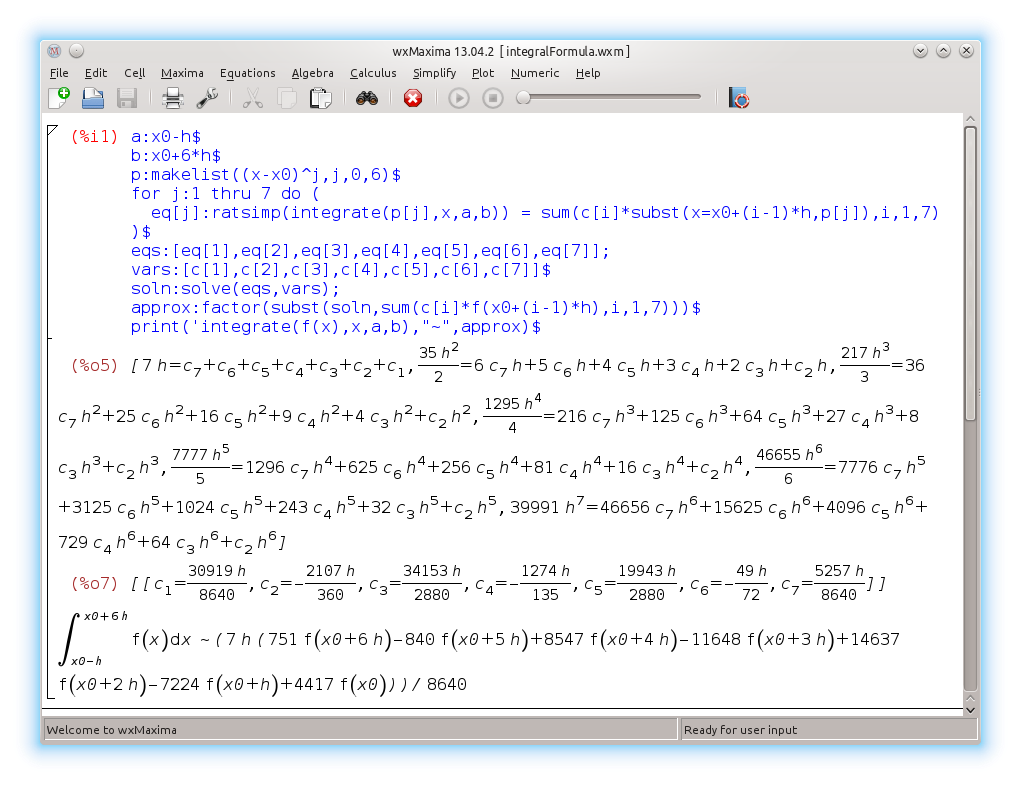
\includegraphics[width=5.5in]{figures/wxmaximaScreenshot}
\end{figure}
 

Pada praktiknya, penggunaan stensil dengan lebih dari lima simpul
memang tidak lazim. Namun, hal ini bukan karena rumus dengan lebih
banyak simpul jauh lebih rumit atau sulit digunakan. Seperti ditunjukkan
oleh rumus \ref{eq:lagrangeInterpolatingPolynomialError}, suku galat
polinom interpolasi melibatkan turunan yang semakin tinggi dari $f$
seiring bertambahnya jumlah simpul. Hal ini umumnya tidak menjadi
masalah selama $f$ memiliki turunan hingga orde yang cukup tinggi
dan nilai turunan berorde tinggi tersebut tidak terlampau besar. Namun,
metode numerik sering digunakan ketika kehalusan $f$ diketahui terbatas,
turunan orde tingginya diketahui bernilai besar, atau sifat-sifat
turunannya sama sekali tidak diketahui. Untuk fungsi-fungsi ini, stensil
dengan lebih sedikit simpul, yang menghasilkan rumus dengan suku galat
berorde lebih rendah, sering kali \textit{lebih akurat}, bukan kurang
akurat. Jika tingkat kehalusannya tidak diketahui, metode berorde
lebih rendah juga memiliki peluang lebih besar untuk tetap akurat.

Sebagai catatan terakhir, kita perlu berhati-hati agar tidak menuntut
terlalu banyak dari suatu rumus turunan. Dengan $n+1$ simpul, suku
galat polinom interpolasi melibatkan $f^{(n+1)}$, sehingga tidak
mungkin menggunakan simpul-simpul ini untuk memperkirakan $f^{(n+1)}$
atau turunan yang lebih tinggi pada titik mana pun. Namun, jika Anda
melupakan fakta ini, hal tersebut akan tampak secara langsung dalam
metode koefisien tak tentu. Jika $k>n$, sistem persamaan dengan koefisien
tak tentu menjadi
\[
\sum_{i=0}^{n}(\theta_{i}h)^{j}a_{i}=0,\qquad j=0,1,\ldots,n
\]
karena turunan orde $k$ dari $p_{j}$ identik nol untuk semua $j\leq n<k$.
Satu-satunya penyelesaian sistem ini adalah $a_{0}=a_{1}=\cdots=a_{n}=0$
sehingga diperoleh rumus ``aproksimasi'' berikut
\[
f^{(k)}(x_{0}+\theta h)=0.
\]
Memang, rumus ini eksak untuk semua polinom berderajat $n$ atau kurang.
Namun, galat akibat penggunaan rumus ini tepat sebesar $f^{(k)}(x_{0}+\theta h)$,
yaitu galat relatif tepat sebesar $1$, sehingga rumus ini sama sekali
tidak berguna.

\subsection{Stabilitas}

Dalam Eksperimen 2 \vpageref{subsec:derivativeExperiment}, bagian
\ref{sec:Accuracy}, kita meninjau secara singkat aproksimasi turunan
pertama $f(x)=\sin x$ dengan menggunakan fakta bahwa
\[
f'(1)=\lim_{h\to0}\frac{\sin(1+h)-\sin(1-h)}{2h}.
\]
Kesimpulan yang kita peroleh adalah bahwa perhitungan ini sangat rentan
terhadap galat titik mengambang. Jika perhitungan dilakukan secara
eksak, kita berharap $\frac{\sin(1+h)-\sin(1-h)}{2h}$ mengaproksimasi
$f'(1)$ dengan semakin baik saat $h$ semakin kecil. Namun, hal ini
tidak berlaku untuk perhitungan titik mengambang, seperti ditunjukkan
oleh eksperimen tersebut. Ada suatu titik ketika memperkecil $h$
justru memperburuk aproksimasi! Contoh ini pun bukan satu-satunya.
Masalah ini selalu muncul ketika mengaproksimasi $f'$ menggunakan
rumus beda terpusat
\begin{equation}
f'(x)\approx\frac{f(x+h)-f(x-h)}{2h}.\label{eq:centeredDifference}
\end{equation}
Namun, bagaimana kita dapat memperkirakan nilai $h$ yang akan memicu
hal itu tanpa membandingkan hasil kita dengan nilai eksak turunannya?
Bagaimanapun, diferensiasi numerik paling sering digunakan ketika
rumus eksak turunannya tidak diketahui atau terlampau sulit untuk
dihitung.

Misalkan $f$ dapat dihitung dengan ketelitian yang mendekati presisi
mesin. Dalam perhitungan titik mengambang biasa, termasuk Octave,
hal itu berarti galat titik mengambang relatif sekitar $10^{-15}$
atau galat titik mengambang mutlak $\varepsilon_{f}\approx10^{-15}|f(x)|$.
Karena kita mengasumsikan $h$ bernilai kecil, kita dapat mengaproksimasi
baik $|\tilde{f}(x+h)-f(x+h)|$ maupun $|\tilde{f}(x-h)-f(x-h)|$
dengan $\varepsilon_{f}$ sehingga diperoleh galat mutlak sekitar
$2\varepsilon_{f}$ dalam menghitung pembilang $f(x+h)-f(x-h)$. Dengan
mengasumsikan $h$ dihitung secara eksak, kita memperoleh galat mutlak
\begin{equation}
\varepsilon_{r}=|\tilde{f}'(x)-f'(x)|\approx\frac{2\varepsilon_{f}}{2h}=\frac{\varepsilon_{f}}{h}=\frac{|f(x)|}{10^{15}}\cdot\frac{1}{h}.\label{eq:floatingPointError}
\end{equation}
Seperti yang akan segera kita lihat, galat algoritmik, $\varepsilon_{a}$,
disebabkan oleh pemotongan dan bernilai $\left|\frac{f'''(\xi)}{6}h^{2}\right|$
untuk suatu nilai $\xi$ di dekat $x$. Karena $\xi$ berada di dekat
$x$, kita mengaproksimasi $f'''(\xi)$ dengan $f'''(x)$ dan menyimpulkan
bahwa 
\begin{equation}
\varepsilon_{a}\approx\frac{|f'''(x)|}{6}h^{2}.\label{eq:algorithmicError}
\end{equation}
Sekarang kita meminimumkan nilai $\varepsilon_{r}+\varepsilon_{a}$
dengan menetapkan turunannya (terhadap $h$) sama dengan nol dan menyelesaikan
persamaan yang dihasilkan:
\begin{eqnarray*}
0=\frac{d}{dh}(\varepsilon_{r}+\varepsilon_{a}) & \approx & \frac{d}{dh}\left(\frac{|f(x)|}{10^{15}}\cdot\frac{1}{h}+\frac{|f'''(x)|}{6}\cdot h^{2}\right)\\
 & = & -\frac{|f(x)|}{10^{15}}\cdot\frac{1}{h^{2}}+\frac{|f'''(x)|}{3}\cdot h\\
 & \Rightarrow\\
\frac{|f'''(x)|}{3}\cdot h & \approx & \frac{|f(x)|}{10^{15}}\cdot\frac{1}{h^{2}}\\
h^{3} & \approx & \frac{|f(x)|}{|f'''(x)|}\cdot\frac{3}{10^{15}}\\
h & \approx & \sqrt[3]{\frac{3|f(x)|}{|f'''(x)|}}\cdot10^{-5}.
\end{eqnarray*}
Untuk Eksperimen 2 \vpageref{subsec:derivativeExperiment}, ini berarti
kita memperkirakan bahwa nilai optimal $h$ berada di sekitar$\sqrt[3]{\frac{3\sin(1)}{\sin(1)}}\cdot10^{-5}\approx1.44(10)^{-5}$.
Kita tampilkan kembali tabel dari Eksperimen 2 di sini dengan menambahkan
kolom ketiga, yaitu galat mutlak sebenarnya:

\begin{center}
\begin{tabular}{c|c|c}
$h$ & $\tilde{p}^{*}(h)$ & $|\tilde{p}^{*}(h)-f'(1)|$\tabularnewline
\hline 
$10^{-2}$ & $0.5402933008747335$ & $9.00(10)^{-6}$\tabularnewline
$10^{-3}$ & $0.5403022158176896$ & $9.00(10)^{-8}$\tabularnewline
$10^{-4}$ & $0.5403023049677103$ & $9.00(10)^{-10}$\tabularnewline
$10^{-5}$ & $0.5403023058569989$ & $1.11(10)^{-11}$\tabularnewline
$10^{-6}$ & $0.5403023058958567$ & $2.77(10)^{-11}$\tabularnewline
$10^{-7}$ & $0.5403023056738121$ & $1.94(10)^{-10}$\tabularnewline
\end{tabular}
\par\end{center}

\noindent Memang, ketika $h=10^{-5}$, kita memperoleh hasil terbaik!
Namun, prediksi nilai optimal untuk $h$ didasarkan pada pengetahuan
tentang $f'''$, sesuatu yang umumnya tidak dapat kita ketahui. Kecuali
jika kebetulan kita mengetahui bahwa $\frac{|f(x)|}{|f'''(x)|}$ jauh
dari $1$, kita mengasumsikan nilainya cukup dekat dengan $1$; dalam
hal ini, nilai optimal $h$ berada di sekitar $10^{-5}$. Perkiraan
serupa dapat dibuat untuk rumus turunan lainnya.

Karena diferensiasi numerik sangat peka terhadap galat titik mengambang,
kita menyebutnya tidak stabil. Metode pencarian akar dan integrasi
numerik yang telah kita bahas semuanya merupakan metode yang stabil.
Kepekaannya terhadap galat titik mengambang sebanding dengan kepekaan
dalam menghitung $f$.

\subsection{Konsep Kunci}
\begin{description}
\item [{koefisien~tak}] tentu: \index{koefisien tak tentu}Metode untuk
menyelesaikan masalah yang bentuk penyelesaiannya telah diketahui,
kecuali sejumlah koefisien yang belum ditentukan.
\end{description}
\noindent\startexercises 

\subsection{Latihan}
\begin{enumerate}
\item \label{exc:undetermined}Dengan menggunakan metode koefisien tak tentu,
turunkan rumus aproksimasi untuk turunan pertama pada stensil tersebut.

\begin{enumerate}
\item \raisepic{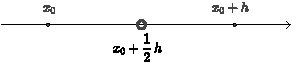
\includegraphics{figures/calculus-undetermined01}}\medskip 
\item \raisepic{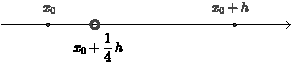
\includegraphics{figures/calculus-undetermined06}} \hasananswer\medskip 
\item \raisepic{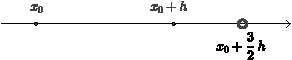
\includegraphics{figures/calculus-undetermined07}}\medskip 
\item \raisepic{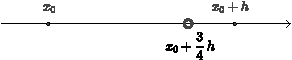
\includegraphics{figures/calculus-undetermined08}} \hasasolution\medskip 
\item \raisepic{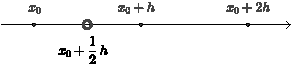
\includegraphics{figures/calculus-undetermined02}}\medskip 
\item \raisepic{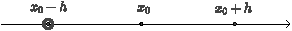
\includegraphics{figures/calculus-undetermined03}} \hasananswer\medskip 
\item \raisepic{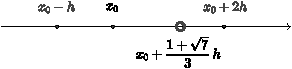
\includegraphics{figures/calculus-undetermined04}}\medskip 
\item \raisepic{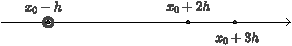
\includegraphics[width=5cm]{figures/calculus-undetermined05}} \hasananswer\medskip 
\item \raisepic{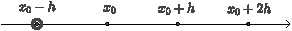
\includegraphics{figures/calculus-undetermined09}}\medskip 
\item \raisepic{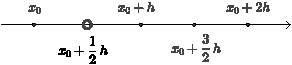
\includegraphics{figures/calculus-undetermined10}} \hasasolution\medskip 
\item \raisepic{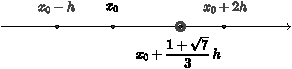
\includegraphics{figures/calculus-undetermined11}}\medskip 
\item \raisepic{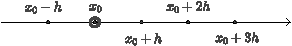
\includegraphics{figures/calculus-undetermined12}} \hasananswer
\end{enumerate}
\item \label{exc:undetermined-1}Dengan menggunakan metode koefisien tak
tentu, turunkan rumus aproksimasi untuk turunan kedua pada stensil
tersebut.

\begin{enumerate}
\item \raisepic{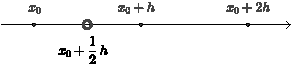
\includegraphics{figures/calculus-undetermined02}}\medskip 
\item \raisepic{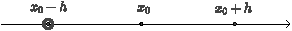
\includegraphics{figures/calculus-undetermined03}} \hasananswer\medskip 
\item \raisepic{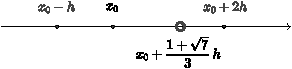
\includegraphics{figures/calculus-undetermined04}}\medskip 
\item \raisepic{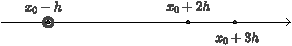
\includegraphics[width=5cm]{figures/calculus-undetermined05}} \hasananswer\medskip 
\item \raisepic{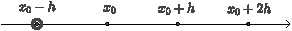
\includegraphics{figures/calculus-undetermined09}}\medskip 
\item \raisepic{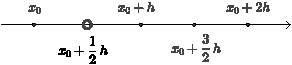
\includegraphics{figures/calculus-undetermined10}} \hasasolution\medskip 
\item \raisepic{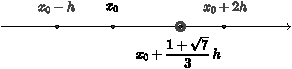
\includegraphics{figures/calculus-undetermined11}}\medskip 
\item \raisepic{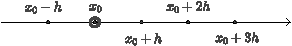
\includegraphics{figures/calculus-undetermined12}} \hasananswer 
\end{enumerate}
\item Gunakan metode koefisien tak tentu untuk menurunkan rumus aproksimasi
pada stensil berikut

\begin{center}
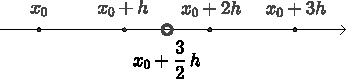
\includegraphics{figures/calculus-rudiments07}
\par\end{center}
\begin{enumerate}
\item untuk nilai fungsi.
\item untuk turunan pertama.
\item untuk turunan kedua.
\item untuk turunan ketiga. Apa yang dapat Anda simpulkan tentang rumus
ini?
\item Bandingkan metode koefisien tak tentu dengan metode langsung yang
digunakan pada soal \ref{exc:rudiments-28} di bagian \ref{sec:NumericalRudiments}.
\end{enumerate}
\item \label{exc:undetermined-2}Gunakan metode koefisien tak tentu untuk
menurunkan rumus aproksimasi untuk integral pada stensil berikut.

\begin{enumerate}
\item \raisepic{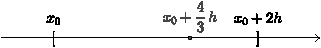
\includegraphics{figures/calculus-undetermined13}}\medskip
\item \raisepic{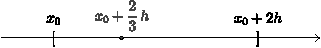
\includegraphics{figures/calculus-undetermined14}} \hasasolution\medskip
\item \raisepic{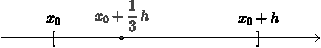
\includegraphics{figures/calculus-undetermined15}}\medskip
\item \raisepic{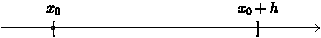
\includegraphics{figures/calculus-undetermined16}} \hasananswer\medskip
\item \raisepic{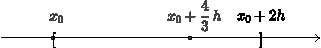
\includegraphics{figures/calculus-rudiments16}}\medskip
\item \raisepic{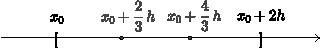
\includegraphics{figures/calculus-rudiments17}} \hasananswer\medskip
\item \raisepic{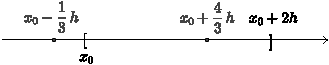
\includegraphics{figures/calculus-rudiments19}}\medskip
\item \raisepic{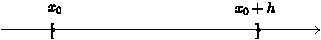
\includegraphics{figures/calculus-rudiments20}} \hasananswer\medskip
\item \raisepic{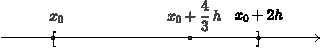
\includegraphics{figures/calculus-undetermined17}}\medskip
\item \raisepic{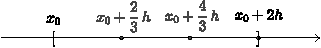
\includegraphics{figures/calculus-undetermined18}} \hasananswer\medskip
\item \raisepic{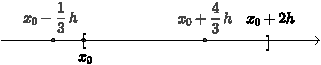
\includegraphics{figures/calculus-undetermined19}}\medskip
\item \raisepic{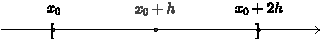
\includegraphics{figures/calculus-undetermined20}} \hasasolution\medskip
\item \raisepic{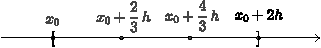
\includegraphics{figures/calculus-undetermined21}}
\end{enumerate}
\item Dengan menggunakan metode koefisien tak tentu, tentukan rumus aproksimasi
umum untuk ${\displaystyle \int_{x_{0}+\theta_{0}h}^{x_{0}+\theta_{1}h}f(x)dx}$
dengan menggunakan dua simpul $x_{0}+\theta_{2}h$ dan $x_{0}+\theta_{3}h$.
\end{enumerate}
\noindent\finishexercises 
